\documentclass[../main/main]{subfiles}

\setcounter{chapter}{4}
\begin{document}

\chapter{設計変数の適応的離散化手法}
\section{設計変数の離散化の課題と解決に向けたアプローチ}
\quad 前章「設計変数の離散化による影響評価」で述べたように,実数値GAにおいて,設計変数を粗く離散化するほど解の収束性が向上する傾向があることが確認された.
しかしながら,問題によっては粗く離散化しすぎると解の収束性・多様性が悪化してしまう場合もあるため,単に粗く離散化された設計変数を用いるだけでは効率的探索は実現できない.
そのため,問題に応じて各設計変数を適切に離散化することで,解の多様性を維持しながらも収束性を向上させることができると考えられる.
しかし,最適化を行う前に事前に各設計変数を適切に離散化することは難しく,設計変数の離散化の活用を応用する課題として残されていた.

そこで本研究では,この課題を解決するアプローチとして設計変数の適応的離散化手法を提案する.
設計変数の適応的離散化手法を用いることで,最適化の中で適切と考えられる離散化を施し,事前に適切な離散化が施せない場合でも効率的に探索できることが期待される.

\section{適応的離散化手法について}
\quad 本研究の適応的離散化手法では,各世代での設計変数空間における解の分布状態によって離散化する大きさを決定することを考える.
進化の過程における解の分布状態は,概ね\Figref{concept_image}に示すように設計変数空間に疎に分布している状態(\Figref{concept_image}(a))から,密に分布している状態(\Figref{concept_image}(b))に遷移していくものと考えられる.

\begin{figure}[htbp]
\begin{tabular}{cc}
\begin{minipage}{0.49\hsize}
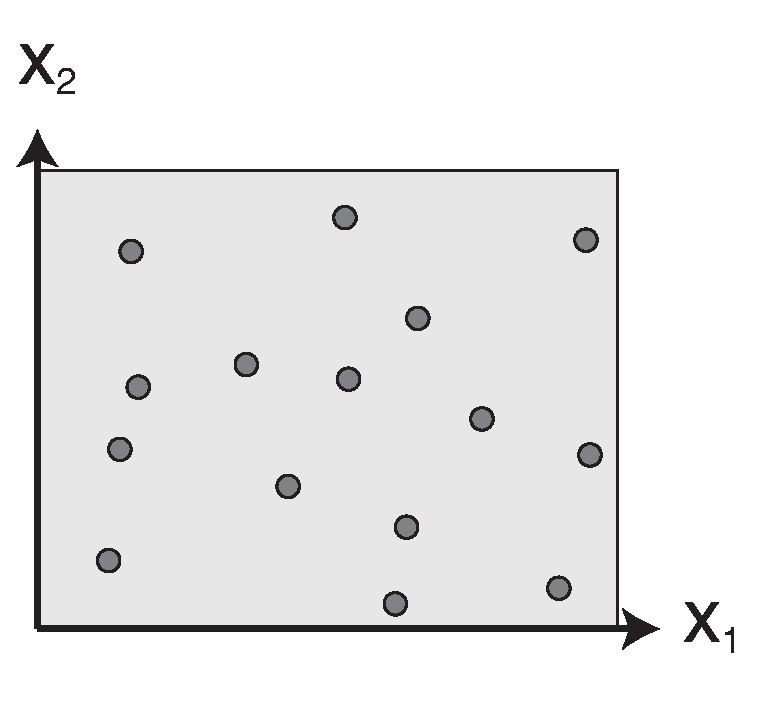
\includegraphics[width=0.9\linewidth]{../figures/sparse_distribution.eps}
\begin{center}
{\footnotesize (a) 疎に分布}
\end{center}
\end{minipage}
\begin{minipage}{0.49\hsize}
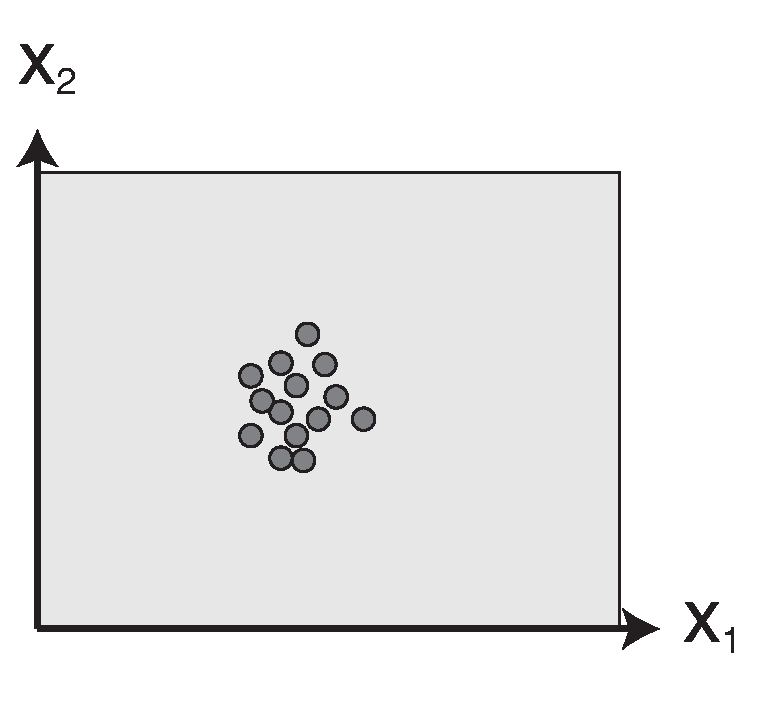
\includegraphics[width=0.9\linewidth]{../figures/dense_distribution.eps}
\begin{center}
{\footnotesize (b) 密に分布}
\end{center}
\end{minipage}
\end{tabular}
\caption{二変数空間での解の分布状態のイメージ図}
\label{concept_image}
\end{figure}

そこで\Figref{concept_image}(a)の場合はまだ設計変数が最適な値に収束していないため粗く離散化し,\Figref{concept_image}(b)の場合はその周辺に最適な解があるため細かく離散化する,という制御を行うことを考える.
このことにより進化初期には粗く離散化することで,大域的探索性能が向上して収束性が加速され,最適解周辺に解が集まるにつれて細かい離散化に自動的に切り替わり,局所探索性能が向上して多様性も維持されることが期待される.
本研究の適応的離散化は,集団の解の分布が求めることができれば適用することができるため,アルゴリズムに依存せずどの実数値GAにも適用可能である.
本研究では実数値GAとしてNSGA-IIを用い,解の分布状態の評価指標としては標準偏差(standard deviation; SD),もしくは,推定された確率密度関数値(estimated probability density function; ePDF)を用いた.
提案手法を適用したNSGA-IIのアルゴリズムをAlgorithm\ref{alg1}に示す.

\vspace{-0.1in}
\begin{algorithm}[t]         
\caption{NSGA-II Algorithm with Proposed Method}         
\label{alg1}                          
\begin{algorithmic}[1]             
\STATE Initialize parent population ($P_0$)
\STATE \underline{Discretize {\rm each} design variable according to solution distribution of $P_0$}\\\underline{ (Proposed method)}
\STATE Evaluate $P_0$
\FOR{${\rm each} \ t = 0, \cdots , t_{\rm max}$}
\STATE Make parent pairs from the population ($P_t$) by the tournament selection
\STATE Conduct a crossover (SBX) and a mutation (polynomial mutation) to generate an offspring population ($Q_t$)
\STATE \underline{Discretize each design variable according to solution distribution of $Q_t$}\\ \underline{ (Proposed method)}
\STATE Evaluate $Q_t$
\STATE Combine $P_t$ and $Q_t$ into $R_t$
\STATE Make a new parent population($P_{t+1}$) from $R_t$ (non-dominated sorting and crowding distance sorting)
\ENDFOR
\end{algorithmic}
\end{algorithm}

初期集団($P_0$)生成後,初期集団の分布から解の分布状態の評価指標(SDまたはePDF)に基づいて各設計変数値を離散化した値に修正し,目的関数及び制約条件の評価を行う.
次に親個体ペアを選択し,交叉と突然変異を行って子個体集団($Q_0$)を生成する.
生成された子個体集団の分布から解の分布状態の評価指標(SDまたはePDF)を計算し,子個体の各設計変数値を離散化した値に修正し,評価を行う.
その後,非優越ソートと混雑距離を用いて親集団を更新する.
本研究では,他のGAにも容易に実装に可能となることや,離散化の影響のみを評価することができることから,内部的に連続値を保持して評価時のみ離散化するのではなく,実際に変数の値を修正する実装とした.
また,解の分布状態の評価には親集団ではなく子集団を用いている.
子集団は,交叉や突然変異の影響により,親集団よりもばらつきの大きな分布となりやすいと考えられる.
提案手法ではばらつきの大きな分布ほど粗く離散化されることから,大域的探索能力が向上して収束師が加速することが期待される.
そこで本研究では標準偏差の計算に子集団を用いることとした.

また,本研究では,設計変数空間を均等に分割し離散化を行うことを考え,設計変数空間を [0,1] の正規化空間に射影し,その値の小数点以下の桁数を制御することで設計変数空間の分割数を決定する.
そのため,離散化に用いるパラメータは制御する小数点以下の桁数$d$となり,設計変数空間の分割数は$10^d$となる.

次節以降で各評価指標を用いた適応的離散化手法を述べる.

\subsection{標準偏差を用いた離散化手法}
\quad 本研究では,設計変数空間の解の分布状態を評価する指標の一つとして標準偏差(standard deviation; SD)を用いる.
SDは\Figref{concept_image}(a)のように疎な分布が得られた場合は大きな値となり,\Figref{concept_image}(b)のように密な分布が得られた場合は小さな値となることから,このSDの値の差を利用し,適応的に離散化することを考える.
SDを用いた制御桁数$d$の算出式を\Eqref{sd_formulation}に示す.

\begin{equation}
d_i = round \left ( \left(1 - \cfrac{\sigma_i}{\sigma_{\rm max}} \right) (d_{\rm max} - d_{\rm min} ) + d_{\rm min} \right )
\label{sd_formulation}
\end{equation}

$d_{i}$は,設計変数$x_i$の制御を行う桁数,$d_{\rm max}$,$d_{\rm min}$は桁数の上限値,下限値を示すパラメータであり,いずれも整数値である.
また,$\sigma_{i}$は設計変数$x_i$の標準偏差,$\sigma_{\rm max}$は最も疎な分布の標準偏差を示しいる.
ここでは,最も疎な分布として一様分布を仮定する.
そのため,$\sigma_{\rm max}$は一様分布の標準偏差となり,0-1の正規化空間について考えるため,$1 / \sqrt{12}$の固定値となる.
\eqref{sd_formulation}式を用いることで,設計変数$x_i$が\Figref{concept_image}(a)のように疎に分布している場合,$\sigma_{i}$は$\sigma_{\rm max}$の値に近づき,$d_{\rm min}$が出力されるため,粗い離散化に切り替わる.
粗い離散化に切り替えることで,大域的探索能力が向上し,解の収束性が加速することが期待される.
逆に,設計変数$x_i$が\Figref{concept_image}(b)のように密に分布している場合,$\sigma_{i}$は$0$に近づき,$d_{\rm max}$が出力されるため,細かい離散化に切り替わる.
細かい離散化に切り替わることで,局所的探索能力が向上し,解の多様性が改善することが見込まれる.


\subsection{推定された確率密度関数値を用いた離散化手法}
\quad 本研究では,設計変数空間の解の分布状態を評価する指標の一つとして推定された確率密度関数値(estimated probability density function; ePDF)を用いる.
ここでは,確率密度関数の推定法としてkernel density estimation (KDE) を用いる.
ePDFを用いることによって,SDでは評価が難しい分布に対しても適切に評価を行うことができる可能性がある.
\Figref{kde_hist}(a)は二変数空間に密な分布が複数存在する場合を示している.
このように密な分布が複数あった場合,SDはスカラー値で評価を行うため,適切に評価することができない可能性がある.
一方で,ePDFを用いるとこのような分布が得られた場合にも適切に評価することができる可能性がある.
\Figref{kde_hist}(b)は(a)の変数$x_1$について,定義域内における頻度ヒストグラムとKDEによって推定されたPDFを示したものである.
灰色のバーは各領域での頻度ヒストグラムを示しており,推定されたPDFは青色の線で示してある.
\Figref{kde_hist}(b)より,青線で示したPDFは,密な分布がある領域で高い値となっており,複数密な分布があるという特徴をうまく捉えることができている.
ePDFは,\Figref{kde_hist}(b)からも分かるように,疎な分布が得られた場合はその付近の領域で小さい値となり,密な分布が得られた場合はその付近の領域で高い値となることから,このePDF値を利用し,探索空間内を部分的かつ適応的に離散化することができると考えた.
ePDFを用いた制御桁数$d$の算出式を\Eqref{epdf_formulation}に示す.

\begin{figure}[t]
\begin{tabular}{cc}
\begin{minipage}{0.35\hsize}
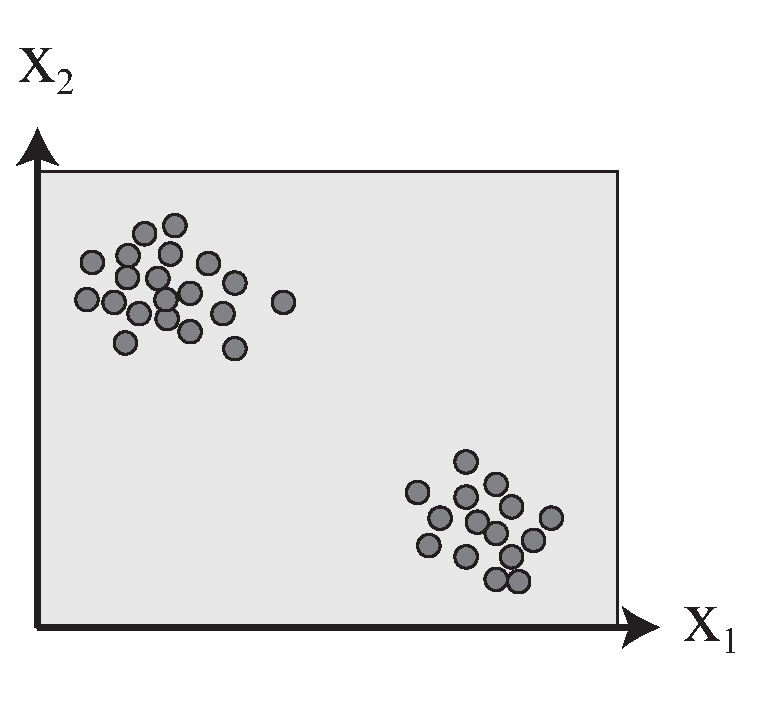
\includegraphics[width=0.95\linewidth]{../figures/mitsu_2.eps}
\begin{center}
\hspace{-0.3in}{\footnotesize (a) 設計変数空間における複数の密分布}
\end{center}
\end{minipage}
\begin{minipage}{0.64\hsize}
\includegraphics[width=0.95\linewidth]{../figures/KDE_hist.eps}
\begin{center}
\hspace{-0.3in}{\footnotesize (b) (a)の$x_1$における頻度ヒストグラムと推定された確率密度関数}
\end{center}
\end{minipage}
\end{tabular}
\vspace{0.1in}
\centering
\includegraphics[width=0.65\linewidth]{../figures/KDE_hist_discretization.eps}\\
%\vspace{0.2in}
\hspace{-0.3in}{\footnotesize (c) 推定された確率密度関数の適応的離散化への適用}
\caption{推定された確率密度関数の利用}
\label{kde_hist}
\end{figure}

\begin{equation}
d_{i,j} = round \left ( \left(1 - \cfrac{\hat{f}_{\rm K}(x_{i,j})}{\mymax_{x{}\in{}[0,1]}\hat{f}_{\rm K}(x)} \right) (d_{\rm max} - d_{\rm min} ) + d_{\rm min} \right )
\label{epdf_formulation}
\end{equation}

$d_{i,j}$はある個体$j$における設計変数$x_i$を制御する桁数を示しており,$d_{\rm max}$,$d_{\rm min}$は桁数の上限値,下限値を示すパラメータであり,いずれも整数値である.
$\hat{f}_{\rm K}(x_{i,j})$はある個体$j$の設計変数$x_i$におけるKDEによって推定されたPDF値を示し,$\max_{x \in [0,1]}\hat{f}_{\rm K}(x)$はKDEによって推定されたPDF値の最大値を示している.
この制御式を用いることで\Figref{kde_hist}(c)のように,各設計変数において,密な分布が得られた領域では細かい離散化が行われ,疎な分布が得られた領域では粗い離散化が行われる,といった部分的な適応的離散化が可能となる.
本手法は,SDを用いた適応的離散化手法ではうまく評価できない複数密な分布が発生するような問題に対して,SDより適切に離散化を行い,更なる効率的探索ができることが期待される.

\end{document}